\documentclass[11pt,a4paper]{article}
\usepackage[utf8]{inputenc}
\usepackage[T1]{fontenc}
\usepackage{amsmath}
\usepackage{amsfonts}
\usepackage{amssymb}
\usepackage[left=3.0cm, right=3.0cm, top=3.0cm, bottom=3.0cm]{geometry}
\usepackage{xcolor}
\usepackage{graphicx}
\usepackage{caption}
\usepackage{subcaption}

% include code listings
\usepackage{listings}

% Defining colors for syntax highlighting
\definecolor{codegreen}{rgb}{0,0.6,0}
\definecolor{codegray}{rgb}{0.5,0.5,0.5}
\definecolor{codepurple}{rgb}{0.58,0,0.82}
\definecolor{backcolour}{rgb}{0.95,0.95,0.92}

\lstdefinestyle{mystyle}{
	backgroundcolor=\color{backcolour},   
	commentstyle=\color{codegreen},
	keywordstyle=\color{magenta},
	numberstyle=\tiny\color{codegray},
	stringstyle=\color{codepurple},
	basicstyle=\ttfamily\footnotesize,
	breakatwhitespace=false,         
	breaklines=true,                 
	captionpos=b,                    
	keepspaces=true,                 
	numbers=left,                    
	numbersep=5pt,                  
	showspaces=false,                
	showstringspaces=false,
	showtabs=false,                  
	tabsize=2
}

\lstset{style=mystyle}
\captionsetup[lstlisting]{font={scriptsize}}

% header and footer
\usepackage{fancyhdr}
\pagestyle{fancy}
\fancyhf{}
\lhead{Michele Guadagnini}
\rhead{\today}
\lfoot{Ex 6 - Quantum Information and Computing 2020/2021}
\rfoot{Page \thepage}

\author{Michele Guadagnini - ID 1230663}
\title{\textbf{Exercise 6 \\ Continuous Time-Independent Schr\"odinger Equation}}
\date{\today}

%File names must include your name, exercise number and codewords REPORT, and CODE.
%Example: Ex2-Rossi-REPORT.pdf
%The maximum length of the report is five pages
\begin{document}
\maketitle

\vspace{20pt}
\begin{abstract}
	The aim of this exercise is to solve the continuous time-independent Schr\"odinger equation for the \textit{harmonic oscillator} potential in one dimension and to calculate the resulting \textit{eigenvalues} and \textit{eigenfunctions}. The computational method chosen is the Finite Difference Method.
\end{abstract}

\section{Theory} %Explain briefly the theory you have based your solution on.

The continuous time-independent Schr\"odinger equation for the one dimensional harmonic oscillator can be written in this form:
\begin{equation}
H \psi = E \psi \quad , \quad where: \quad H = -\frac{\hbar^2}{2m}\frac{d^2}{dx^2} + \frac{1}{2}m\omega^2 x^2
\label{eq:SE}
\end{equation}
The eigenvalues of this system are defined as: $E_n = \hbar\omega(n+\frac{1}{2})$.
The eigenfunctions can be expressed by mean of the \textit{Hermite Polynomials}.

%simplification 
We can simplify the problem by setting $\hbar$ and $2m$ to $1$ and the hamiltonian $H$ to:
\begin{equation}
H = -\frac{d^2}{dx^2} + \omega^2 x^2
\label{eq:hamiltonian}
\end{equation}
In this way the expected eigenvalues are: $E_n = 2n+1$.

To solve the problem numerically it is needed to discretize the space in a certain range and also the derivative computation. 
The resulting equation after discretization is:
\begin{equation}
-\frac{1}{h^2}(\psi_{n+1} + \psi_{n-1} - 2\psi_n) + \omega^2 x_{n}^2\psi_n = E_n\psi_n
\label{eq:discreteSE}
\end{equation}
where $h$ is the unit step in the discretized space.
Finally, the eigenpairs can be computed by expressing in matrix form the hamiltonian above and by diagonalizing it. 

\section{Code Development} %Introduce strategies, tests, and report debugging problems, compilations options

\subsection{Design and Implementation}
The code has been split in to files, one containing the module with all the needed subroutines definitions, \textit{Ex6-Guadagnini-ContinuousTimeIndSE-CODE.f90}, and the other, \textit{Ex6-Guadagnini-CODE.f90}, containing the main program.
Also the \textit{Debugger} module has been included in the main program.

The program receives as input $4$ parameters: 
the frequency of the harmonic oscillator, $\omega$; 
the system dimension in unit of $\frac{1}{\omega}$, $width$; 
the number of divisions to perform in the system space, $Ndiv$; 
the number of eigenvalues and eigenvectors to save on file, $k$.

The module file contains the following subroutines:
\begin{itemize}
	\item \textit{InitDefaults}: it sets the default values for the above parameters when command line arguments are not present or invalid. 
	\item \textit{Discretize}: it computes the system dimension $L$, the extremes of the system space in order to have them symmetric with respect to zero, the unit step $h$ and the vector of discretized space points.
	\item \textit{HarmonicOscillatorPot}: it computes the harmonic oscillator potential as defined in the previous section. Separating the computation of the potential allows to easily change it in future by creating a new subroutine for the new potential.
	\item \textit{InitHamiltonian}: it creates the hamiltonian matrix as upper triangular. Indeed, the \textit{DSYEV} subroutine from \textit{LAPACK} does not require the full matrix because it is supposed to be symmetric, as in our case.
	\item \textit{SymmetricEigenpairs}: it performs the diagonalization of the matrix using the subroutine \textit{DSYEV}, returning both eigenvalues and eigenvectors.
	\item \textit{PrintEigVals}: it simply prints in a file two columns with the expected and computed eigenvalues.
	\item \textit{PrintEigVecs}: it normalizes the eigenvectors dividing them by $\sqrt{h}$ and prints them in a file beside the discretized space points.
\end{itemize}

%\lstinputlisting[language=FORTRAN, firstnumber=27, linerange={27-42}]{Ex6-Guadagnini-ContinuousTimeIndSE-CODE.f90}

Finally the main program has been implemented, that reads the arguments from command line, verifies them to be acceptable and then calls sequentially the subroutines defined above. It also prints some messages to the screen and calls the \textit{debug} subroutines during execution.

\subsection{Debug and Test}
The program can be compiled and executed with the following commands:
\begin{lstlisting}[language=BASH,numbers=none]
gfortran *CODE.f90 -o ContTimeIndSE.x -lblas -llapack  
./ContTimeIndSE.x 1 10 1001 20
\end{lstlisting}
Also some optimization flags has been tested without any problem, but without significant improvements in computation time, since the heavier calculations are done by the \textit{DSYEV} subroutine, which is already optimized in the code.

In order to obtain meaningful results, care must be used when setting the input parameters. 
Generally, it can be said that increasing the number of division $Ndiv$ improves the computation accuracy, while the $width$ parameter must be not too small to allow the eigenfunctions to go to zero on the edges. 

\section{Results} %Present data and explain your results.
After some tests, the command and parameters used to produce the results presented in this section are:
\begin{lstlisting}[language=BASH,numbers=none]
./ContTimeIndSE.x 1 25 2001 80
\end{lstlisting}

Table \ref{tab:eigvals} reports the first 80 computed eigenvalues.
It can be noticed that the first eigenvalue is very close to the expected value, while the greater eigenvalues tends to have a greater error.
The same consideration can be done by looking at Figure \ref{fig:EigValsErr} that shows the percentage relative error of the computed eigenvalues. 
The relative error seems to increase linearly until $137$, where it starts to decrease rapidly, crossing the zero line for the eigenvalue $147$ and worsening itself very fast.

Finally, Figure \ref{fig:EigFuncs} shows as an example the first four approximated eigenfunctions.
 
% Table snippet
\begin{table}
	\begin{center}
		\begin{tabular}{cc|cc|cc}
			\hline
			\textbf{Expected} & \textbf{Computed} & \textbf{Expected} & \textbf{Computed} & \textbf{Expected} & \textbf{ Computed} \\ \hline
			        1         &    0.99999023     &        55         &    54.98522064    &        109        &    108.9419515     \\
			        3         &    2.99995117     &        57         &    56.98412644    &        111        &    110.93980134    \\
			        5         &    4.99987304     &        59         &    58.98299314    &        113        &    112.93761208    \\
			        7         &    6.99975585     &        61         &    60.98182075    &        115        &    114.93538376    \\
			        9         &    8.99959959     &        63         &    62.98060926    &        117        &    116.93311654    \\
			       11         &    10.99940426    &        65         &    64.97935868    &        119        &    118.93081083    \\
			       13         &    12.99916987    &        67         &    66.97806899    &        121        &    120.92846775    \\
			       15         &    14.9988964     &        69         &    68.9767402     &        123        &    122.9260902     \\
			       17         &    16.99858387    &        71         &    70.97537231    &        125        &    124.92368549    \\
			       19         &    18.99823226    &        73         &    72.97396532    &        127        &    126.92127103    \\
			       21         &    20.99784157    &        75         &    74.97251922    &        129        &    128.91888679    \\
			       23         &    22.99741182    &        77         &    76.97103402    &        131        &    130.91662027    \\
			       25         &    24.99694298    &        79         &    78.96950971    &        133        &    132.91465378    \\
			       27         &    26.99643508    &        81         &    80.9679463     &        135        &    134.91334776    \\
			       29         &    28.99588809    &        83         &    82.96634377    &        137        &    136.91337474    \\
			       31         &    30.99530202    &        85         &    84.96470213    &        139        &    138.91591224    \\
			       33         &    32.99467687    &        87         &    86.96302139    &        141        &     140.922881     \\
			       35         &    34.99401265    &        89         &    88.96130153    &        143        &    142.93717682    \\
			       37         &    36.99330934    &        91         &    90.95954255    &        145        &    144.96280141    \\
			       39         &    38.99256694    &        93         &    92.95774447    &        147        &    147.00478354    \\
			       41         &    40.99178546    &        95         &    94.95590726    &        149        &    149.06883168    \\
			       43         &    42.9909649     &        97         &    96.95403094    &        151        &    151.16077089    \\
			       45         &    44.99010524    &        99         &    98.9521155     &        153        &    153.2859264     \\
			       47         &    46.9892065     &        101        &   100.95016095    &        155        &    155.44864445    \\
			       49         &    48.98826867    &        103        &   102.94816727    &        157        &    157.65206631    \\
			       51         &    50.98729175    &        105        &   104.94613447    &        159        &    159.8981537     \\
			       53         &    52.98627574    &        107        &   106.94406254    &                   &                    \\ \hline
		\end{tabular}
	\end{center}
	\caption{First 80 eigenvalues obtained from the computation.}
	\label{tab:eigvals}
\end{table} 

%% figure
\begin{figure}
    \centering
	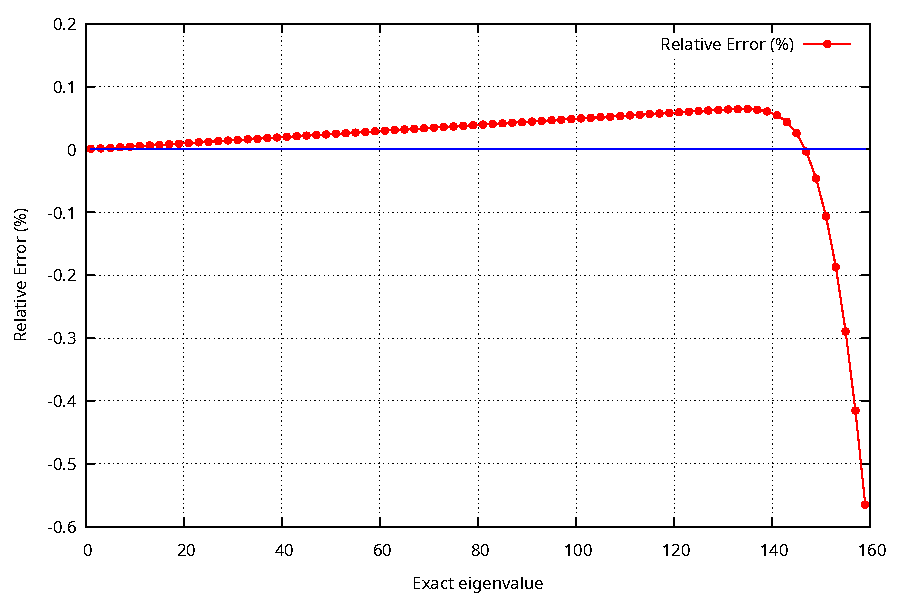
\includegraphics[width=0.95\linewidth]{EigenvaluesError.pdf}
	\caption{Percentage relative error of the first 80 computed eigenvalues.}
	\label{fig:EigValsErr}
\end{figure}

\begin{figure}
	\centering
	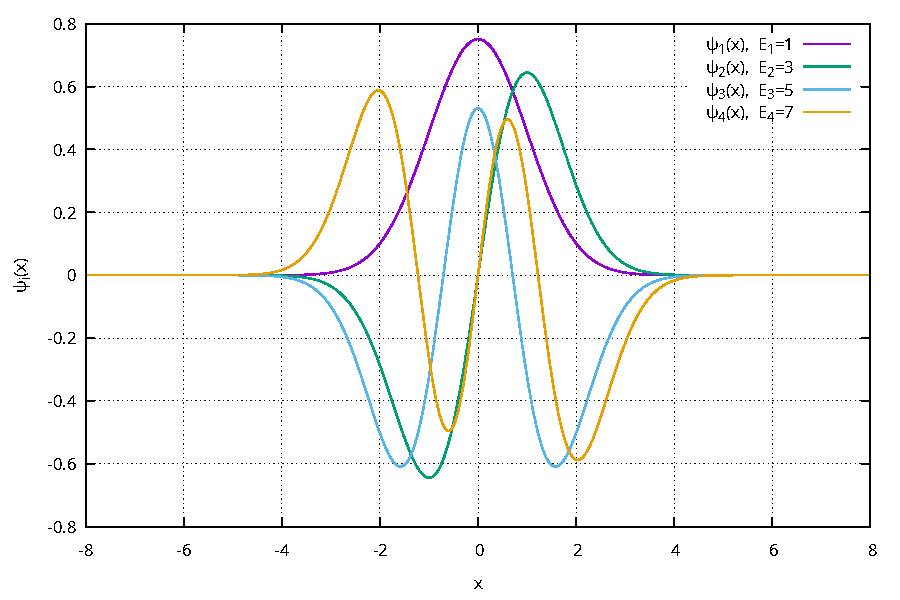
\includegraphics[width=0.95\linewidth]{Eigenfunctions.pdf}
	\caption{First four approximated eigenfunctions. In the legend is reported also the corresponding exact eigenvalue.}
	\label{fig:EigFuncs}
\end{figure}

\section{Self-evaluation} %What have you learned? What can be done next? What went wrong and why?

This program is rated in the following way with respect to the five priorities introduced in class about writing good software:
\begin{itemize}
	\item \textit{Correctness}: the program seems overall correct and it also performs some checks on variables values, but probably it can be improved in exception handling and with pre- and post- conditions.
	\item \textit{Numerical Stability}: in the program all the hard-coded real variables has been set explicitly with double precision (for example by writing $1d0$ instead of $1$). 
	Also the conversions between types has been done explicitly with double precision function (for example using \textit{DFLOAT()} instead of \textit{FLOAT()}). 
	However, Figure \ref{fig:EigValsErr} suggests the presence of some error accumulation.
	\item \textit{Accurate Discretization}: the space has been discretized symmetrically with respect to zero; this showed better accuracy in the results, probably because the harmonic potential is an even function. 
	\item \textit{Flexibility}: the program has been split in smaller parts that eventually allow to build a new program by reusing the same subroutines or by changing one of these. 
	For example the potential computation has been separated from the hamiltonian matrix building in order to make easier to set a different potential. 
	Also, by using command line arguments it allows to change some parameters without the need to recompile the program.
	One thing that could have been done is to make the \textit{Discretize} subroutine receive in input also the extremes of the space to be discretized, allowing to use also potentials not centered at zero.
	\item \textit{Efficiency}: the heaviest calculation are done by the \textit{DSYEV} subroutine to diagonalize the matrix, which is part of the \textit{LAPACK} library. 
	Different optimization flags has been tested without useful improvements.
	When possible, vectorized operations has been preferred against hand-coded loops.
\end{itemize}
	
\end{document}
